\chapter{Design and construction of experimental apparatus}
\label{beamline}

\section{Introduction}
\label{intro_beamline}


\section{Beamline}
\label{sec:full_beamline}
\begin{figure}
	\centering
	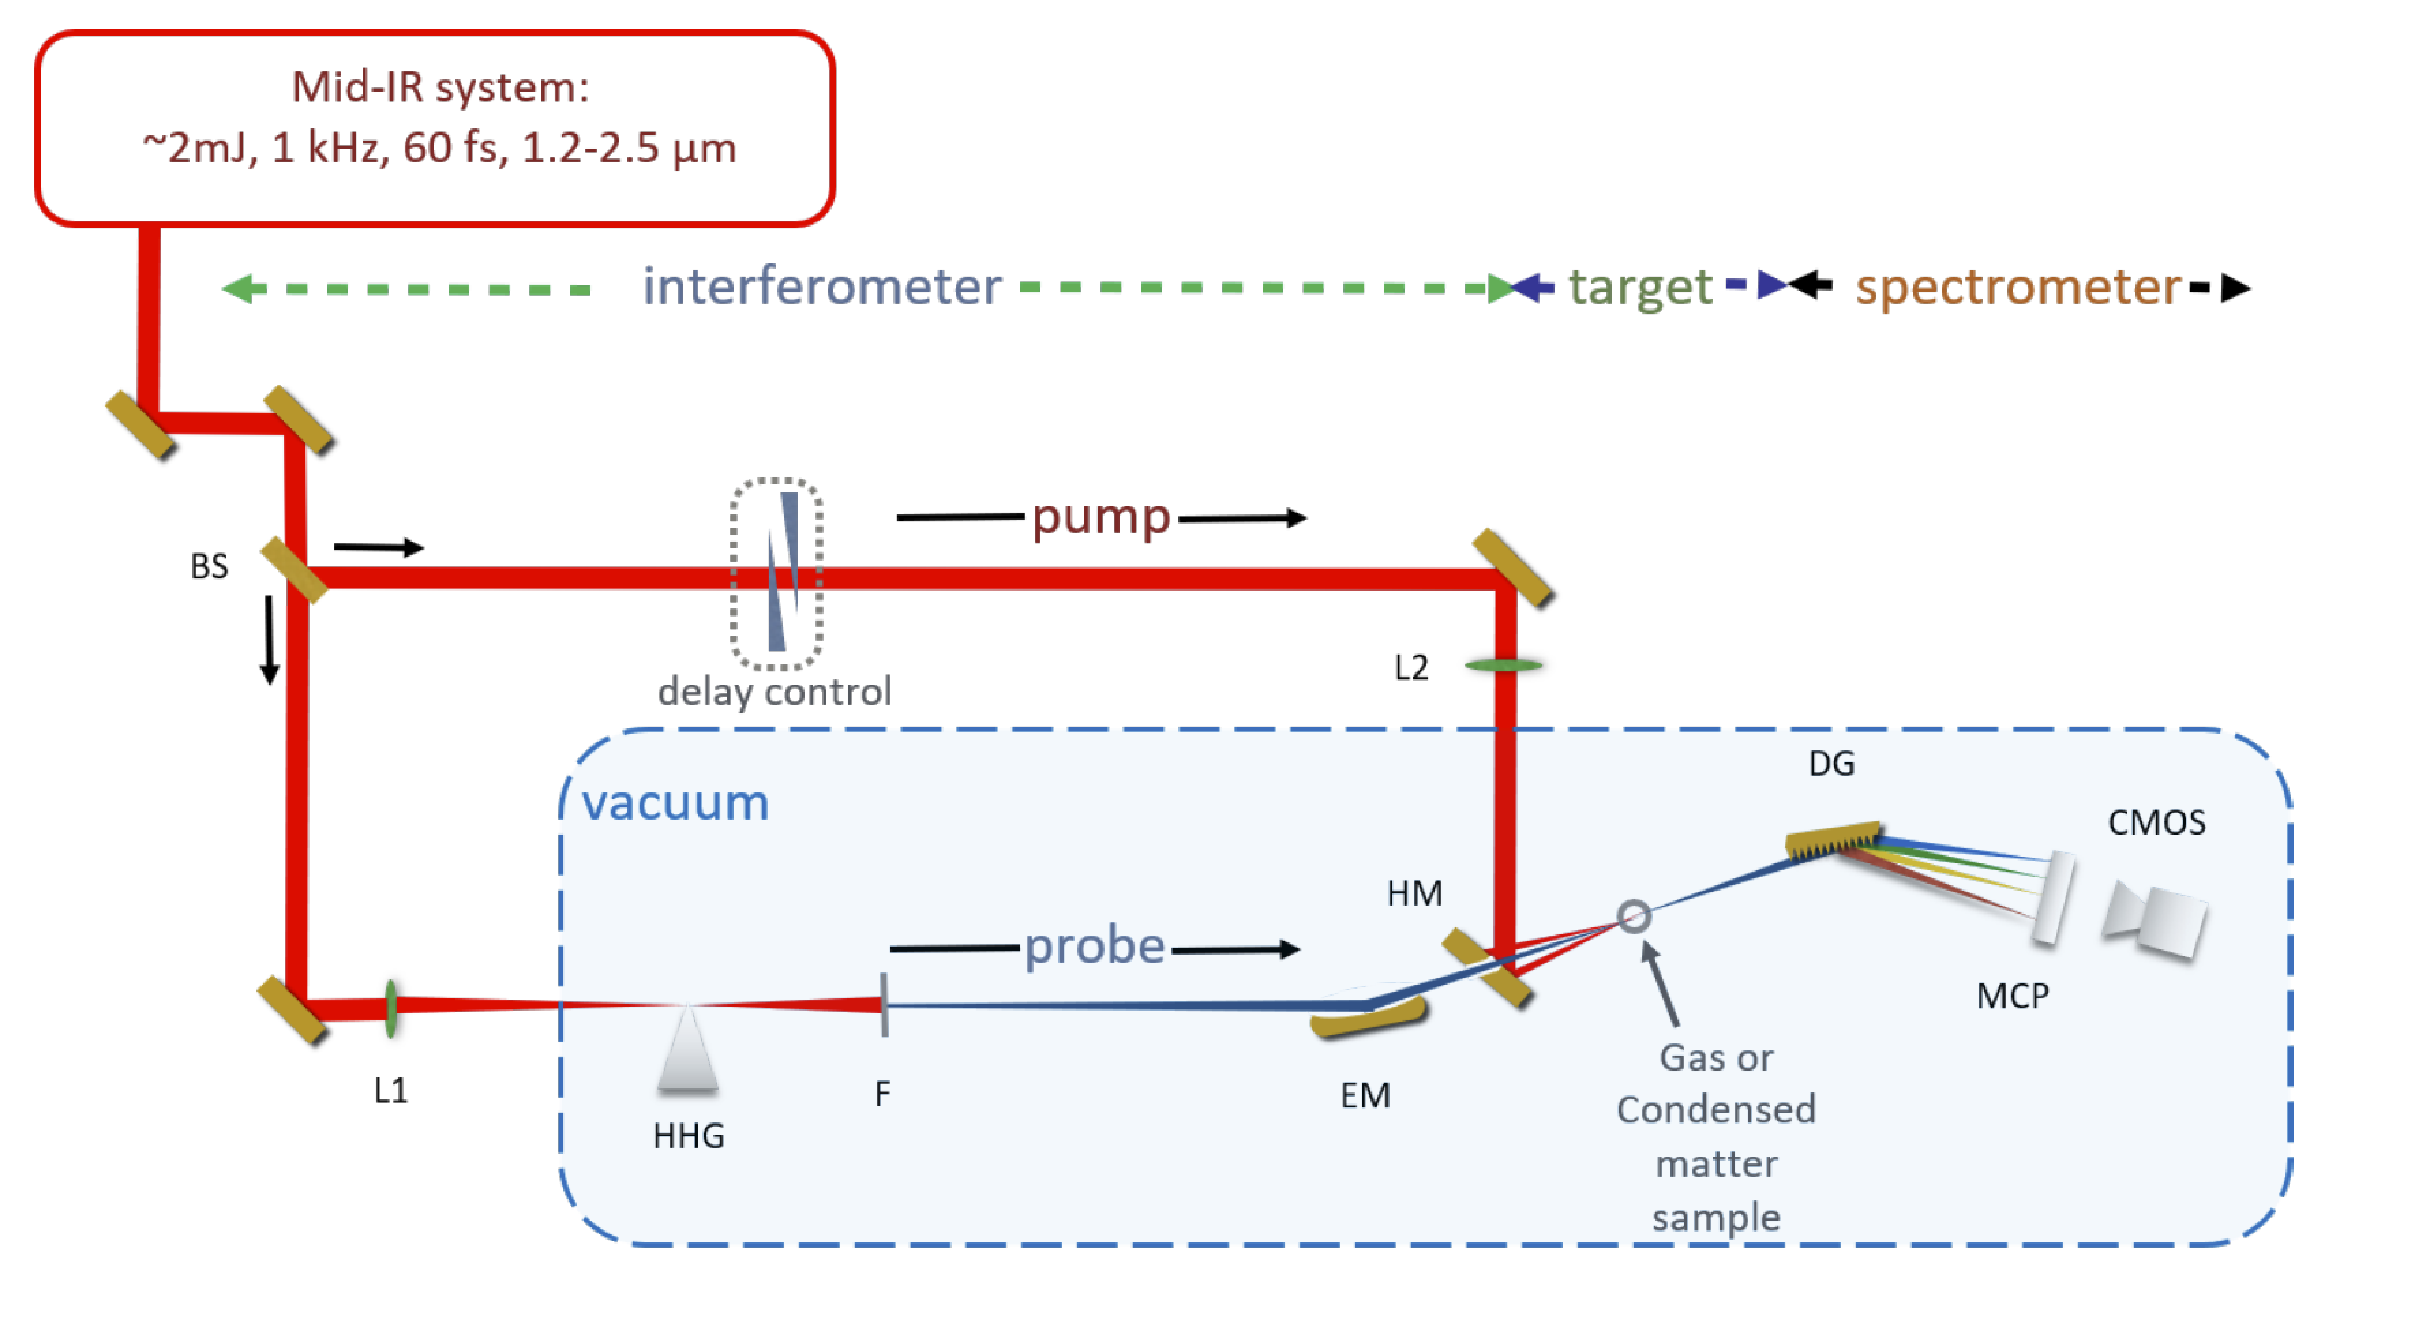
\includegraphics[width=0.8\textwidth]{figures/Beamline/beampath_sketch.pdf}
	\caption{Incomplete schematic of beampath}
	\label{fig:beampath_sketch}
\end{figure}
\subsection{Time Delay Control}
\label{sec:delay_wedges}

An important consideration in pump/probe experiments is how to control the delay between the pump and probe pulses.  To control this delay, there are typically two methods that can be employed optically.  The first to to use a retro-reflector that is mounted on a motorized stage \cite{jagerAttosecondTransientAbsorption2018, jagerAttosecondTransientAbsorption2017, bellTransientAbsorptionSpectroscopy2013, jiangChargeCarrierDynamics2015, borjaElectronDynamicsSolids2016, chengAttoseondTransientAbsorption2015}.  With this method, the delay is simply related to the displacement of the motorized stage by the relationship $\Delta\tau = 2\Delta x/c$.  This means that a displacement of 10 nm by the motorized stage would lead to a delay of 67 as, whereas a displacement of 2 in. would lead to a delay of 339 ps. This setup is advantageous if large delays are required (10s of ps to a few ns), however for the short time steps that are required for an attosecond measurement (typically on the order of 100 as) the requirements on the motor being used to move the retro are very high.  Since a 100 as step would equate to a translation of 15nm, this would require the use of a piezoelectric motor.  Piezo motors and their associated electronics tend to be expensive, and they have inherent problems because they exhibit nonlinear movement due to hysteresis and they tend to drift and creep after actuation.  This can be abated through a feedback sensor and operating it in a closed-loop mode, however the quality of the sensor and electronics determines how effectively these problems are minimized.

\begin{figure}
	\centering
	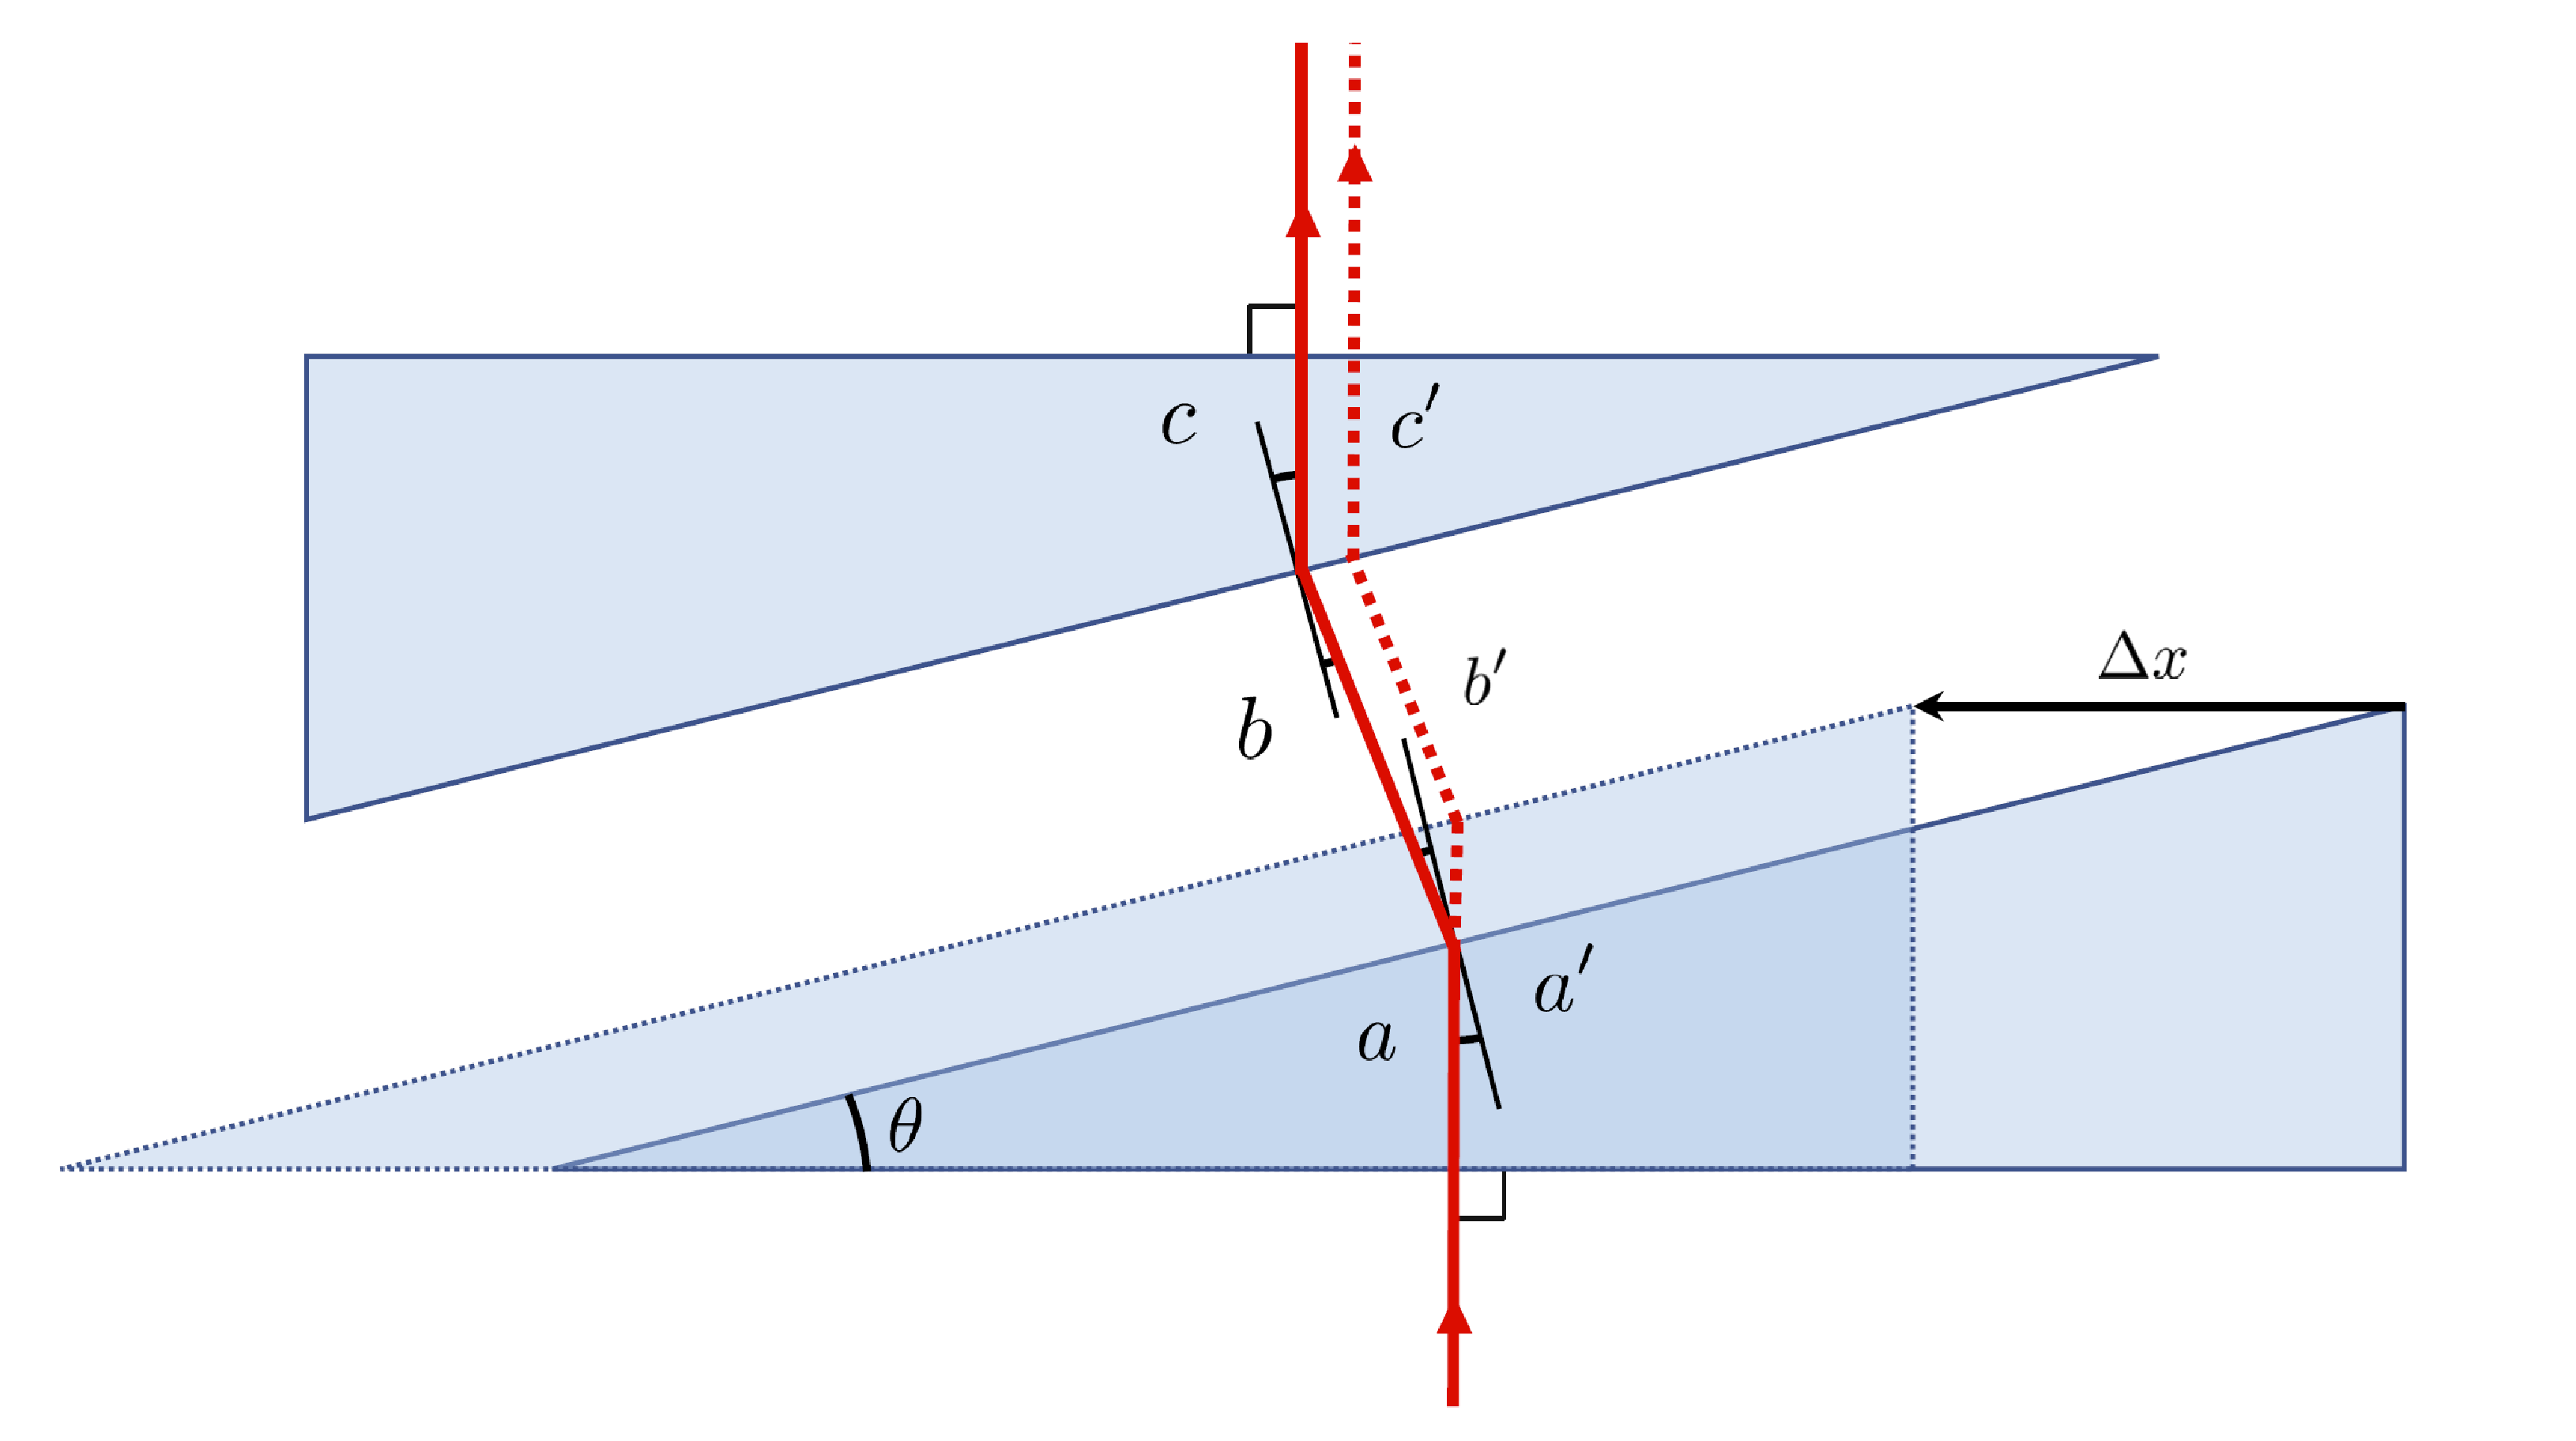
\includegraphics[width=0.9\textwidth]{figures/Beamline/wedge_calibration.pdf}
	\caption{Schematic of the FS wedges used to control the time delay between the IR and XUV pulses in the dressing and generation arms interferometer, respectively. The wedges are aligned such that the input beam is normal to the first wedge face, and the beam exits the wedges normal to the last face of the second wedge.  Only one of the wedges is motorized and is shown before and after a displacement by an amount $\Delta x$.}
	\label{fig:wedges}
\end{figure}

The second common method to control the delay between the pump and probe pulse is to use a pair of glass wedges \cite{chirlaAttosecondPulseGeneration2011, gormanAttosecondProbingElectron2018, kiesewetterDynamicsNearThresholdAttosecond2019}. A schematic of how this is achieved is shown in figure \ref{fig:wedges}.  In this scheme, only one of the glass wedges is motorized, and the direction of translation is perpendicular to the input beam and parallel to the first glass face.  The path that a ray would take through the wedge pair is shown before ($a\rightarrow b\rightarrow c$) and after ($a' \rightarrow b'\rightarrow c'$) translation by an amount $\Delta x$.  Assuming that the wedge angle is $\theta$, the path after translation by $\Delta x$ can be written as
\begin{align}
\label{eqn:path_lengths}
	a'&=a+\Delta x \tan\theta\\
	b'&=b-\Delta x \bigg(\frac{\sin\theta}{\cos\psi}\bigg)\\
	c'&=c-\Delta x \tan\theta\sin\theta\frac{\cos(\frac{\pi}{4}+\psi)}{\sin(\frac{\pi}{4}+\theta+\psi)}
\end{align}
where
\begin{equation}
	\psi = \arcsin(n\sin\theta)
\end{equation}
is given by Snell's Law \cite{pedrottiIntroductionOptics2007}. From the difference in optical path length between these two paths, one can calculate the time delay $\Delta\tau$ introduced by a translation of $\Delta x$, and this relationship is given by
\begin{equation}
\label{eqn:time_delay}
	\Delta\tau = \frac{\Delta x}{c}\Bigg[(n-1)\tan\theta - \frac{\sin\theta}{\cos\psi}-(n-1)\tan\theta\sin\theta\bigg(\frac{\cos(\frac{\pi}{4}+\psi)}{\sin(\frac{\pi}{4}+\theta+\psi)}\bigg)\Bigg].
\end{equation}
For a pair wedges made out of fused silica with a wedge angle of $\theta=5^\circ$ and a beam of wavelength 1430 nm, equation \ref{eqn:time_delay} becomes
\begin{equation}
\label{eqn:numerical_relationship_wedges}
	\Delta\tau = \Bigg(101 \bigg[\frac{\mathrm{as}}{\mathrm{\mu m}}\bigg]\Bigg)\Delta x.
\end{equation}
This entails that a translation of 1 $\mu$m would lead to a delay of only 100 as.  This reduction in motor step to delay step ratio compared to the retroreflector case means that the requirements on the motorized stage are greatly reduced.  Additionally, since the glass wedges are a transmissive optic, they are inherently less sensitive to vibrations when compared to a retroreflector.

In the TABLe apparatus, both types of delay control have been implemented, as shown in figure \ref{fig:beampath_sketch}.  The retroreflector is mounted on a translation stage with 2 inches of travel that is controlled manually with a micrometer.  The primary use for the retroreflector is to make coarse adjustments to the dressing arm to account for changes in temporal overlap between the two arms of the interferometer.  Typically, this is due to adjustments made to the interferometer itself (such as introducing new optics) or due to changes in the input laser, usually either pointing or wavelength.  

To finely control the delay, a pair of glass wedges is used.  These wedges are made out of fused silica, and have a wedge angle of $\theta=5^\circ$.  The first of the two wedges are motorized in manner similar to that shown in figure \ref{fig:wedges}.  The stage that the first wedge is mounted to has a total travel of 1 inch, and it is controlled by a Thorlabs Z825B DC servo motor.  This "pencil" motor, as it is known in the lab, has a minimum repeatable incremental motion of 0.2 $\mu$m and is encoded, so it's absolute position is known to within the homing accuracy of $\pm1$ $\mu$m.  From equation \ref{eqn:numerical_relationship_wedges}, using these wedges at 1430 nm with a step size of 1 $\mu$m will give a delay of 101 as.

\subsection{Spatial and Temporal Overlap}
\label{sec:temporal_overlap}

\begin{figure}
	\centering
	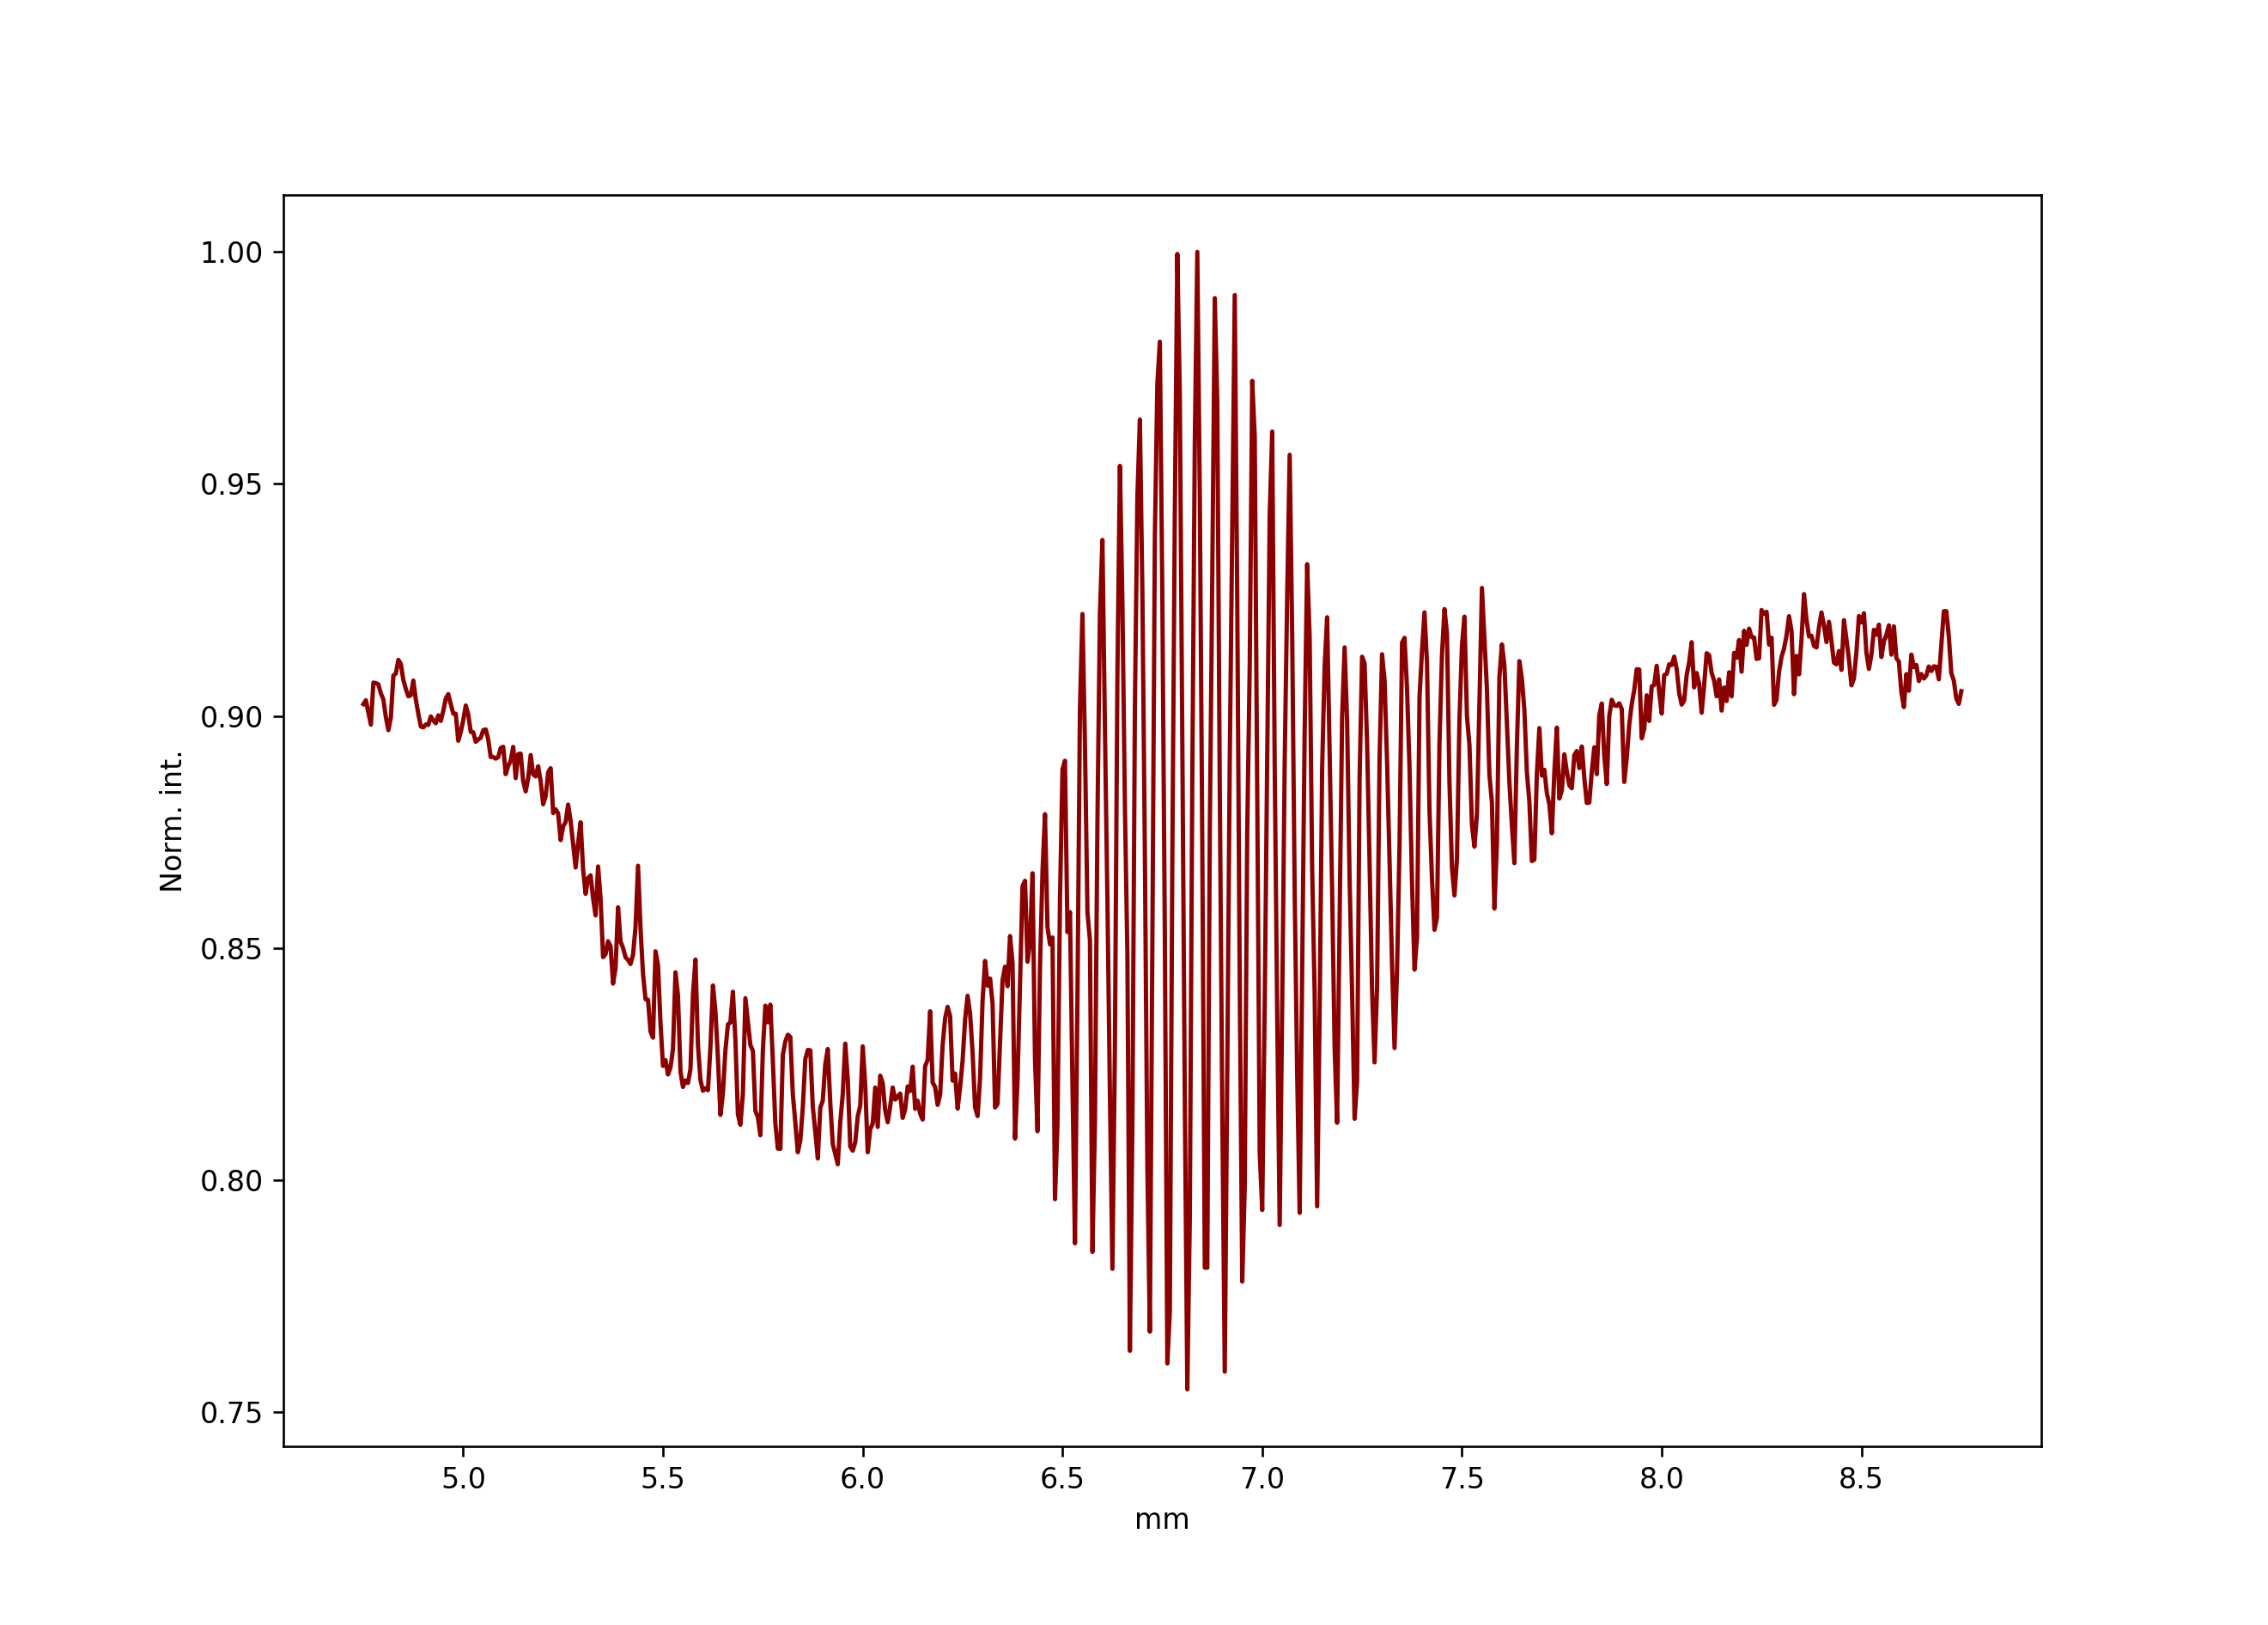
\includegraphics[width=0.9\textwidth]{figures/Beamline/Overlap_camera.png}
	\caption{INCOMPLETE: Autocorrelation to find temporal overlap.}
	\label{fig:fine_scan_temporal_overlap}
\end{figure}

\subsection{IR Dressing Intensity}
\label{sec:dressing_intensity}



\section{Photon Spectrometer}
\label{sec:photon_spec}


\subsection{Spectrometer Calibration}
\label{subsec:spec_calibration}